%%%%%%%%%%%%%%%%%%%%%%%%%%%%%%%%%%%%%%%%%%%%%%%%%%%%%%%%%%%%%%%%%%%%%%%%%%%
% Copyright (c) 2010 committers of YAKINDU and others.
% All rights reserved. This program and the accompanying materials
% are made available under the terms of the Eclipse Public License v1.0
% which accompanies this distribution, and is available at
% http://www.eclipse.org/legal/epl-v10.html
%
% Contributors:
%     committers of YAKINDU - initial API and implementation
%%%%%%%%%%%%%%%%%%%%%%%%%%%%%%%%%%%%%%%%%%%%%%%%%%%%%%%%%%%%%%%%%%%%%%%%%%%
\section{The Generated Source Code}

The Java source code generated by the YAKINDU Statechart Java code generator
consists of a set of generic classes (located within the
\texttt{com.yakindu.statechart} package) and a model specific state chart
implementation class, named according to the respective Statechart, here
\texttt{Traffic\-Light\-Statechart} within \texttt{trafficlight} package),
which is outlined by Figure \ref{fig:screenshot22}. It is the single class
that may be directly used by clients to integrate the generated code with
manually written or other generated code.

To obtain a new instance of the state chart implementation, the generated
implementation class offers a static method named \texttt{createInstance()}.
It returns a completely initialized state chart instance, which may be started
(via \texttt{enter()}), cyclically executed (via \texttt{runCycle()}), and
stopped again (via \texttt{leave()}).

Feeding the state chart with external events is done by passing respective
event constants (declared within the state chart implementation class) into
the state chart instance (via \texttt{setEvent()}) prior to executing a new
cycle (via \texttt{runCyle()}). Setting variable values is similarly possible
via respective selector methods generated into the implementation class (a
pair of getter and setter for each variable of the state chart). On each call
to \texttt{runCycle()}, the state chart reacts on all events currently raised
(since the completion of the prior cycle) and reads the variable values as
they are set when calling \texttt{runCycle()}. After \texttt{runCycle()} has
been completed, all events raised prior to its execution will be cleared and
the variables reflect the values as they result from the reaction of the state
chart.

\begin{figure}[h!]
\center
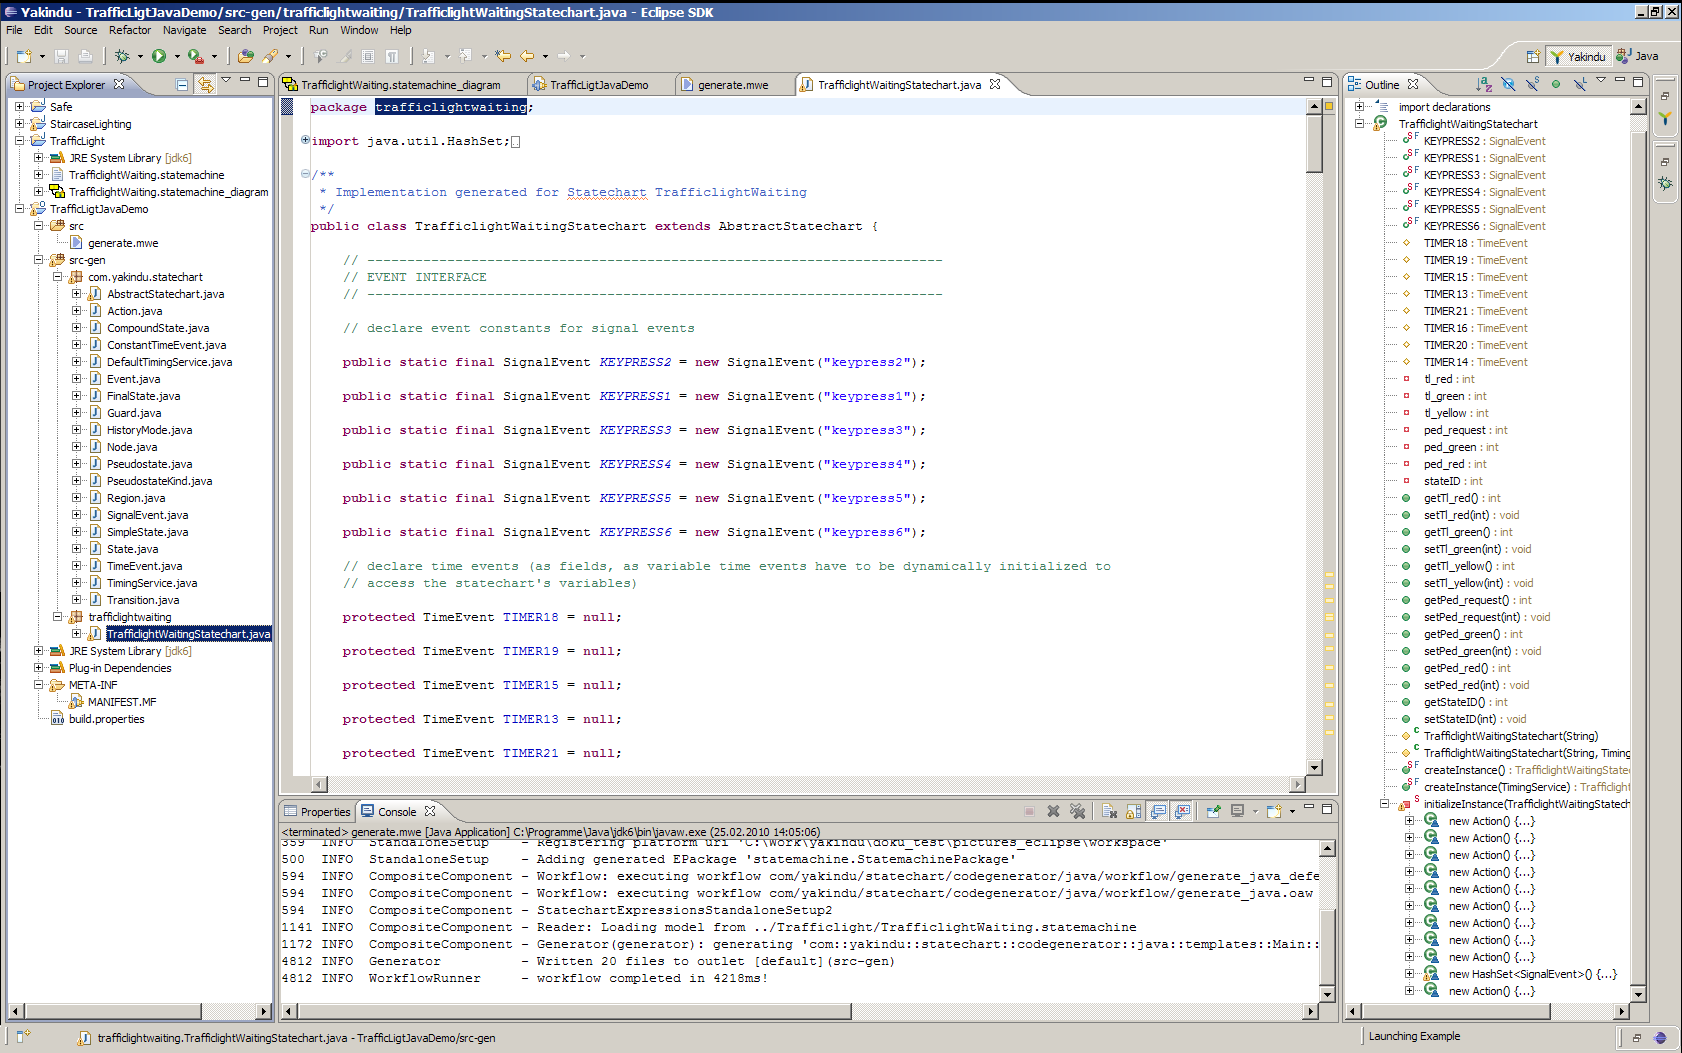
\includegraphics[width=\textwidth]{./Pictures/Screenshot22}
\caption{\label{fig:screenshot22}}
\end{figure}
\clearpage
